\section{Functional Role of Remixing}

The previous section helped describe the structural properties of the Scratch Online Comunity as a remixing system.
This section is intended to examine what people do.
In particular, the goal is to understand what are the different roles remixing plays and how it is part of collaborative and creative practices.

Remixing represents a wide range of activities in Scratch.
For example, in some cases, people remix to fix software bugs on someone's project, in other cases people want to add to an existing project to customize it or make it more personal, in others, people want to start a trend or ``meme'' so they create a ``template'' project just so others remix it, add to it and pass it on.

In order to map out this varied types of remixing, I focus on two dimensions:
\begin{enumerate}
\item{Similarity}. This is how different a remix is from the original work it is based on. 
Remixes can range from merely being inspired by someone's idea, to tweaking someone's project, to making an exact copy.
This is an important aspect of remixing because it gets at the core of some of the tensions around remixing and it also helps us understand the degree of interaction and creative output between a remix and its anteceden project.
\item{Number of people}. This is the number people involved or intended to involved in the remix.
Remixes can range from a single author (e.g. a creator remixing herself as a form of version control), to a small group of people (e.g. a team collaborating in making projects together), to a crowd (e.g. a large group of people participating in a remix chain).
The number of people involved is a useful dimension because it helps us identify very distinct roles remixing plays in Scratch.
\end{enumerate}

Using these two dimensions, one can identify a set of remixing categories (Figure~\ref{fig:function} useful for the analysis of the functional roles of remixing in Scratch.
Broadly speaking, the types of remixing I plan to use to guide my analyses are the following:

\subsection{Incremental Remixing}
This type of remixing often involves downloading someone's project to customize it or fix a bug. 
For example, replacing the costumes of a sprite in a game for a different one. 
This form of remixing often occurs when people make small modifications to the sample projects that come pre-installed with Scratch.
Also, there is anectdotal evidence that suggest that this form of remixing tends to be a useful way newcomers get started with Scratch, who modify an existing project instead of creating a completely new project.
This type of remixing sometimes leads to controversy when the changes are very subtle or non-existent.
Project creators sometimes argue that when the changes are minimal this type of remixing should not be allowed.


\subsection{Component Remixing}
Remixing also occurrs when people, rather than building on top of existing work, use pieces of others' projects to create something new. 
In these cases, often one cannot quickly tell how the remix and the original are related.
This type of remixing typically involve some of the sample sprites that come pre-installed with Scratch, such as the ``jetpack girl'' example mentioned before or some of the templates, images or sounds that members of the community explicitly created for others to reuse.


\subsection{Group Remixing}
Remixing is also used by groups or ``collabs'', as they are often referred to by Scratch members, to work collaboratively by remixing one another's work almost a a form of version control \citep{tichy_rcs_1985}.
For example, in a collab we analyzed before \citep{aragon_tale_2009}, we found that one member of the group would start by creating a first version of the project they had decided to make while others would work on varied parts such as the images, sounds or the engine in the case of a game.
In that collab in particular, there were, on average, 17 remixes before officially releasing a project.
In this case, remixing is part of an explicit collaborative activity.


\subsection{Crowd Remixing}
The home page of the Scratch website has a section called ``What the Community is Remixing''  that features the three top remixed projects in the past two weeks.
While these projects could be represent any type of remixing, they are typically projects that consists of a compelling template that encourages people too add something small to it and pass it on to someone else, like a chain.
For example, one of those projects titled ``Add yourself to the party'' shows a character dancing at a colorful dance floor by itself.
The creator leaves a note in the description of the project inviting people to download the project and add a sprite representing their avatar or profile picture.
Other representative examples are ``Remix if you care about animal rights'', representing a type of crowd remixing with a social cause, and ``Coloring contest'', representing popular genre among more artistic-inclined community members that consists of downloading a still image (often with music playing in then background), coloring it and submitting it to a contest for the best colored image.
While typically the intention of the creator of this type of projects is to create a chain, often the structure of the remix network looks more like a star due to people not following the rules or not checking where the last element of the chain is.
This types of remixes are often incremental like the category described before, but the relationship between the creator and its intended audience is significantly different. 
Crowd remixing explicitly invites people to remix en masse following a specific template. 
The objective of the creation is not the creation itself but the collection of lots of remixes created by many individuals.
There is evidence to suggest that this type crowd remixing emerged after the top remixed projects section was added to the website, but research is needed to understand this phenomena.
\subsection{Inspirational Remxing}
On the far end of the similarity spectrum are projects that are projects inspired by other projects that do not use any particular component of the original work.
These projects are often trying to replicate popular software, video games or even genres that have emerged in the community.
For example, some people create remixes of the Microsoft Windows operating system, or the iPhone, or operating systems that other members of the community have created such as SynOS, a popular Scratch-based pseudo-operating system created by a teenage member of the community.
Other examples of inspirational remixes are the ``fan art'' projects created after popular characters created by other members of the Scratch community such as ``Maki-Tak'', a lizard that dances and sings in animations created by a teenage girl,  or  ``Mr. Happy Man'', a grumpy character invented by a teenage boy.
This type of inspirational remixing is a lot harder to identify automatically since the original and the remix do not share any actual bytes but their names, descriptions and project viewing log data might help. 

\subsection{Self-remixing}
Test account
Versioning

\begin{figure}
\centering
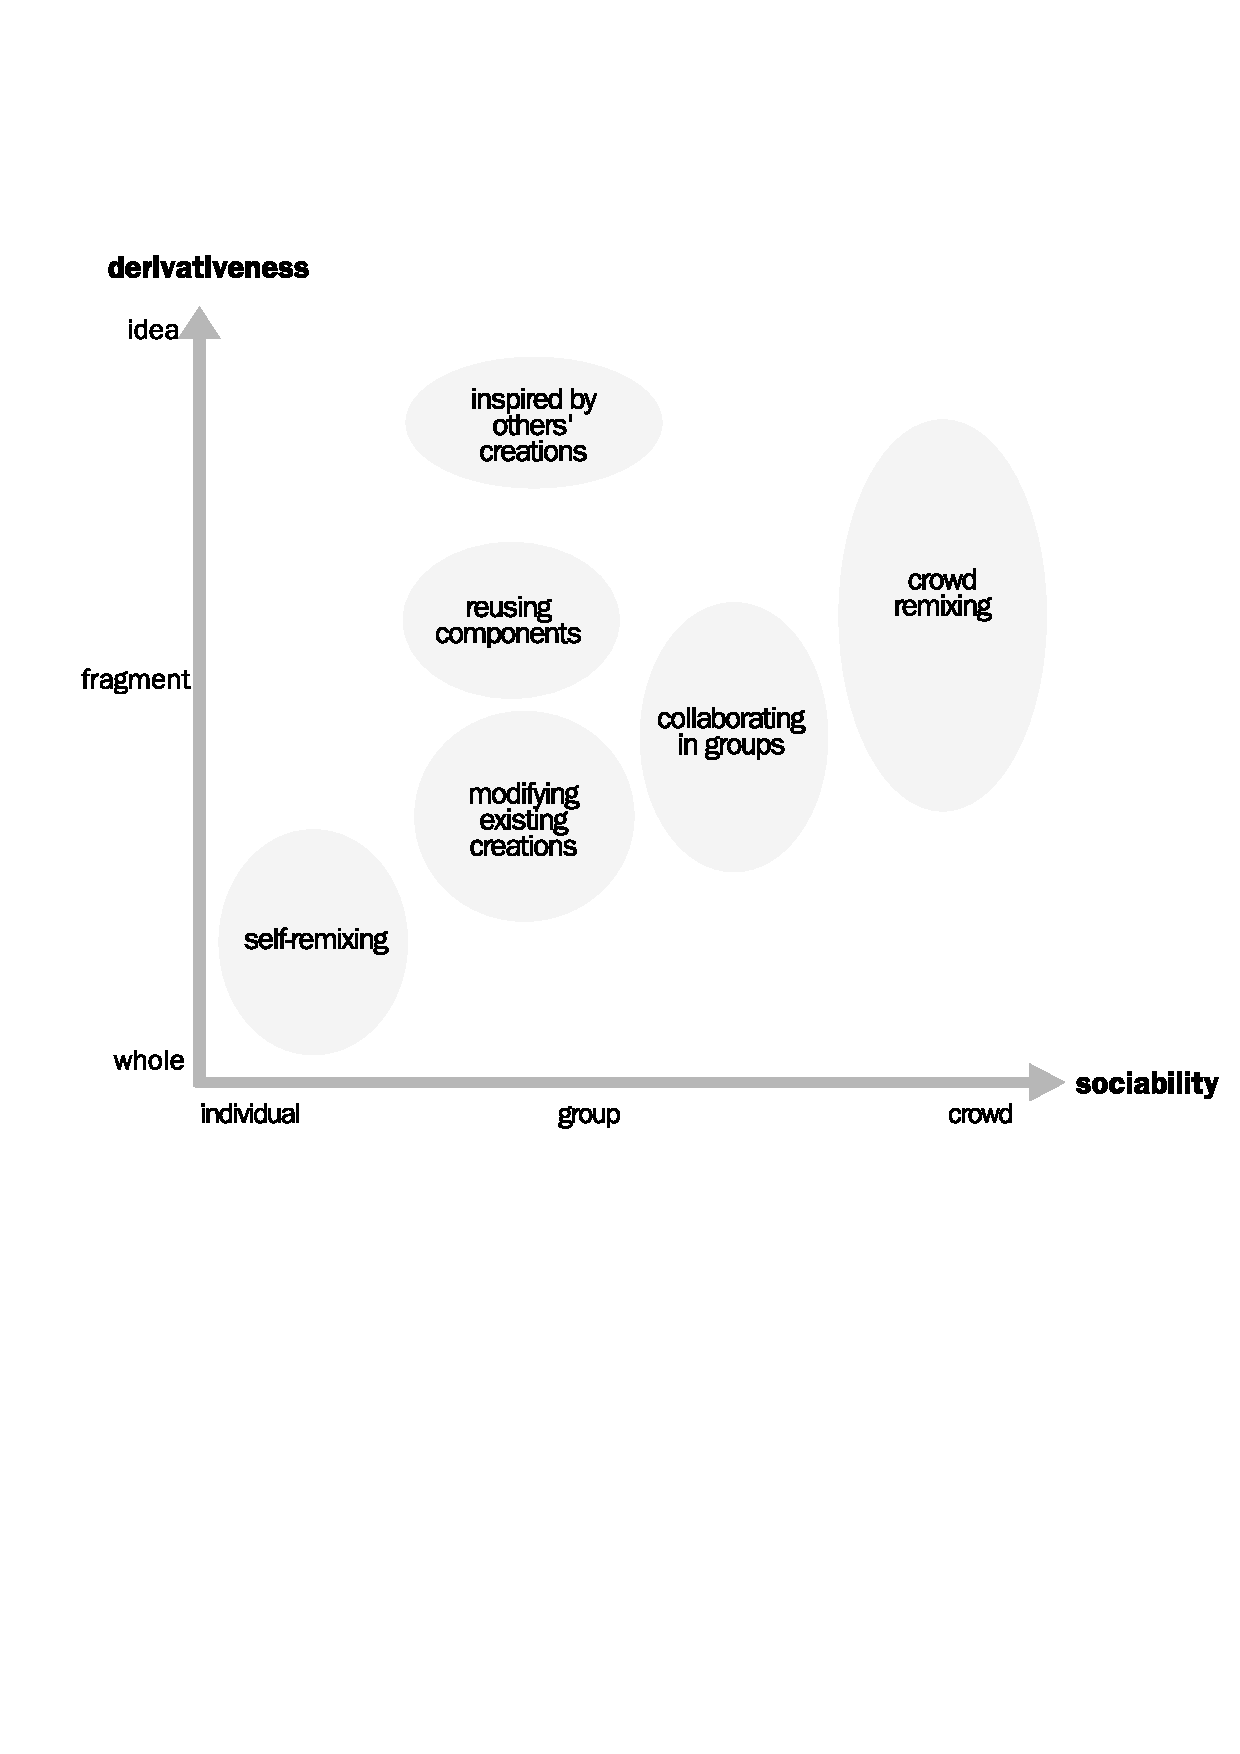
\includegraphics[width=3.25in]{figures/function.pdf}
\caption{Functional roles of remixing in the social and produc-focus dimensions}
\label{fig:function}
\end{figure}
\subsection{Proposed work}
In this section I plan to answer
I plan to answer questions such as:
1. How prevalent is each one of those types of remixing?
2. What kind of people engage in each type of remixing?
3. In what ways do some types of remixing help scaffold Scratch participation? Do they support learning Scratch programming, how to collaborate and socialize with others online?
4. 
% - Evolution of each type.
% - How do they engage in these different forms of production.
% - To what extent do these different forms of remixing support:
% a) scaffolding,  b) committment, c) creative and d) collaborative practices? e) reputation
% 	Look at people who get started by remixing and compare it to those who don't. Follow take other pats.
% 1. Modifying existing work. 
% 4. Crowds: coloring contests
% Some of these roles are analyzed from a network perspective. For example, the network of people engaged in colloring contests represents a group of people involved in a gift exchange network.
% MEASURE OF EFFORT - time to share and number of blocks

In particular, I plan to examine how each category is represented in the Scratch, how their use evolves overtime (in the community as a whole and for each individual user), and how they do or do not support sociability and creative learning.
The distinction is prehaps subjective, part of the work I plan to do is to identify clearer boundaries between each oone of these categories.

